% Options for packages loaded elsewhere
\PassOptionsToPackage{unicode}{hyperref}
\PassOptionsToPackage{hyphens}{url}
\PassOptionsToPackage{dvipsnames,svgnames*,x11names*,table}{xcolor}
%
\documentclass[
  10pt,
  ignorenonframetext,
  aspectratio=43,
]{beamer}
\usepackage{pgfpages}
\setbeamertemplate{caption}[numbered]
\setbeamertemplate{caption label separator}{: }
\setbeamercolor{caption name}{fg=normal text.fg}
\beamertemplatenavigationsymbolsempty

%%
%%% Definition of colors
%%% Source: https://latexcolor.com/
\definecolor{blanchedalmond}{rgb}{1.0, 0.92, 0.8}
\definecolor{blond}{rgb}{0.98, 0.94, 0.75}
%%% End of definition of colors
%%

% Prevent slide breaks in the middle of a paragraph
\widowpenalties 1 10000
\raggedbottom
\usepackage{lmodern}
\usepackage{amssymb,amsmath}
\usepackage{ifxetex,ifluatex}
\ifnum 0\ifxetex 1\fi\ifluatex 1\fi=0 % if pdftex
  \usepackage[T1]{fontenc}
  \usepackage[utf8]{inputenc}
  \usepackage{textcomp} % provide euro and other symbols
\else % if luatex or xetex
  \usepackage{unicode-math}
  \defaultfontfeatures{Scale=MatchLowercase}
  \defaultfontfeatures[\rmfamily]{Ligatures=TeX,Scale=1}
  \setmainfont[]{Fira Sans}
  \setmathfont[]{Fira Math}
  \ifxetex
    \usepackage{xeCJK}
    \setCJKmainfont[ItalicFont=AR PL UKai TW]{AR UDJingXiHeiPU30}
  \fi
  \ifluatex
    \usepackage[]{luatexja-fontspec}
    \setmainjfont[ItalicFont=AR PL UKai TW]{AR UDJingXiHeiPU30}
  \fi
\fi
\usetheme[]{metropolis}
\usecolortheme{default}
\usefonttheme{serif} % use mainfont rather than sansfont for slide text
% Use upquote if available, for straight quotes in verbatim environments
\IfFileExists{upquote.sty}{\usepackage{upquote}}{}
\IfFileExists{microtype.sty}{% use microtype if available
  \usepackage[]{microtype}
  \UseMicrotypeSet[protrusion]{basicmath} % disable protrusion for tt fonts
}{}
\makeatletter
\@ifundefined{KOMAClassName}{% if non-KOMA class
  \IfFileExists{parskip.sty}{%
    \usepackage{parskip}
  }{% else
    \setlength{\parindent}{0pt}
    \setlength{\parskip}{6pt plus 2pt minus 1pt}}
}{% if KOMA class
  \KOMAoptions{parskip=half}}
\makeatother
\usepackage{xcolor}
\IfFileExists{xurl.sty}{\usepackage{xurl}}{} % add URL line breaks if available
\IfFileExists{bookmark.sty}{\usepackage{bookmark}}{\usepackage{hyperref}}
\hypersetup{
  pdftitle={RD Identification Strategy of Women Reserved Seats},
  pdfauthor={Yu-Hsin Ho},
  colorlinks=true,
  linkcolor=Maroon,
  filecolor=Maroon,
  citecolor=Blue,
  urlcolor=red,
  pdfcreator={LaTeX via pandoc}}
\urlstyle{same} % disable monospaced font for URLs
\newif\ifbibliography
\usepackage{listings}
\newcommand{\passthrough}[1]{#1}
\lstset{defaultdialect=sh}
\lstset{framexleftmargin=0mm, frame=trBL,backgroundcolor=\color{blanchedalmond!5},numbers=left,numberstyle=\scriptsize,basicstyle=\small}
\lstset{aboveskip=5mm,belowskip=5mm,xleftmargin=20pt,xrightmargin=5pt}
% \lstset{prebreak={\raisebox{0ex}[0ex][0ex]}}
% \lstset{postbreak={\raisebox{0ex}[0ex][0ex]\space}}
\lstset{breaklines=true,breakatwhitespace=true}
\usepackage{longtable,booktabs}
\usepackage{caption}
% Make caption package work with longtable
\makeatletter
\def\fnum@table{\tablename~\thetable}
\makeatother
\usepackage{graphicx,grffile}
\makeatletter
\def\maxwidth{\ifdim\Gin@nat@width>\linewidth\linewidth\else\Gin@nat@width\fi}
\def\maxheight{\ifdim\Gin@nat@height>\textheight\textheight\else\Gin@nat@height\fi}
\makeatother
% Scale images if necessary, so that they will not overflow the page
% margins by default, and it is still possible to overwrite the defaults
% using explicit options in \includegraphics[width, height, ...]{}
\setkeys{Gin}{width=\maxwidth,height=\maxheight,keepaspectratio}
% Set default figure placement to htbp
\makeatletter
\def\fps@figure{htbp}
\makeatother
\setlength{\emergencystretch}{3em} % prevent overfull lines
\providecommand{\tightlist}{%
  \setlength{\itemsep}{0pt}\setlength{\parskip}{0pt}}
\setcounter{secnumdepth}{-\maxdimen} % remove section numbering

%
% When using babel or polyglossia with biblatex, loading csquotes is recommended 
% to ensure that quoted texts are typeset according to the rules of your main language.
%
\usepackage{csquotes}

%
% blockquote
%
\definecolor{blockquote-border}{RGB}{221,221,221}
\definecolor{blockquote-text}{RGB}{89,89,89}
\usepackage{mdframed}
\newmdenv[rightline=false,bottomline=false,topline=false,linewidth=3pt,linecolor=blockquote-border,skipabove=\parskip]{customblockquote}
\renewenvironment{quote}{\begin{customblockquote}\list{}{\rightmargin=0em\leftmargin=0em}%
\item\relax\color{blockquote-text}\ignorespaces}{\unskip\unskip\endlist\end{customblockquote}}

%
% Source Sans Pro as the de­fault font fam­ily
% Source Code Pro for monospace text
%
% 'default' option sets the default 
% font family to Source Sans Pro, not \sfdefault.
%

\usepackage{adjustbox}
\usepackage{booktabs}
\usepackage{siunitx}
\linespread{1.2}
\usepackage{array}

\title{RD Identification Strategy of Women Reserved Seats}
\author{Yu-Hsin Ho}
\date{Aug 4, 2022}
\institute{Department of Economics, National Taiwan University}

\begin{document}
\frame{\titlepage}

\begin{frame}{席次分配規則:黑爾商數最大剩餘數法}
\protect\hypertarget{ux5e2dux6b21ux5206ux914dux898fux5247ux9ed1ux723eux5546ux6578ux6700ux5927ux5269ux9918ux6578ux6cd5}{}
\begin{enumerate}
\tightlist
\item
  計算分配一名額的人口基數:\textbf{縣市}人口數÷應選名額
\item
  算出選區可以分多少人:FLOOR(選區人口數÷人口基數)
\item
  不足基數的選區分配一名
\item
  餘數由大排到小,每選區分一名,至總應選人數達到規定為止
\end{enumerate}
\end{frame}

\begin{frame}
\begin{block}{例:2010 年新北市議會選舉}
\protect\hypertarget{ux4f8b2010-ux5e74ux65b0ux5317ux5e02ux8b70ux6703ux9078ux8209}{}
\begin{enumerate}
\tightlist
\item
  總人口數:3844081;應選市議員人數:62 人
\item
  每席議員的人口基數:\(3844081 \div 62 = 62001\)
\end{enumerate}

\begin{longtable}[]{@{}cccc@{}}
\toprule()
選區 & 人口數 & 分配席次 & 餘數 \\
\midrule()
\endhead
1 & 211027 & 3 & 25024 \\
2 & 631667 & 10 & 11657 \\
3 & 583784 & 9 & 25775 \\
4 & 550663 & 8 & 54655 \\
5 & 411860 & 6 & 39854 \\
6 & 234200 & 3 & 48197 \\
7 & 588362 & 9 & 30353 \\
8 & 333314 & 5 & 23309 \\
9 & 70120 & 1 & 8119 \\
10 & 229084 & 3 & 43081 \\
\midrule()
& 3844081 & 57 & \\
\bottomrule()
\end{longtable}
\end{block}
\end{frame}

\begin{frame}
\begin{longtable}[]{@{}cccccc@{}}
\toprule()
選區 & 人口數 & 餘數 & 分配席次 & 餘數分配 & 最終席次 \\
\midrule()
\endhead
\rowcolor{blond} 4 & 550663 & 54655 & 8 & 1 & 9 \\
\rowcolor{blond} 6 & 234200 & 48197 & 3 & 1 & 4 \\
\rowcolor{blond} 10 & 229084 & 43081 & 3 & 1 & 4 \\
\rowcolor{blond} 5 & 411860 & 39854 & 6 & 1 & 7 \\
\rowcolor{blond} 7 & 588362 & 30353 & 9 & 1 (cutoff) & 10 \\
3 & 583784 & 25775 & 9 & & 9 \\
1 & 211027 & 25024 & 3 & & 3 \\
8 & 333314 & 23309 & 5 & & 5 \\
2 & 631667 & 11657 & 10 & & 10 \\
9 & 70120 & 8119 & 1 & & 1 \\
\bottomrule()
\end{longtable}
\end{frame}

\begin{frame}{應選 \(3 \rightarrow 4\);保障 \(0 \rightarrow 1\)}
\protect\hypertarget{ux61c9ux9078-3-rightarrow-4ux4fddux969c-0-rightarrow-1}{}
\begin{figure}
\centering
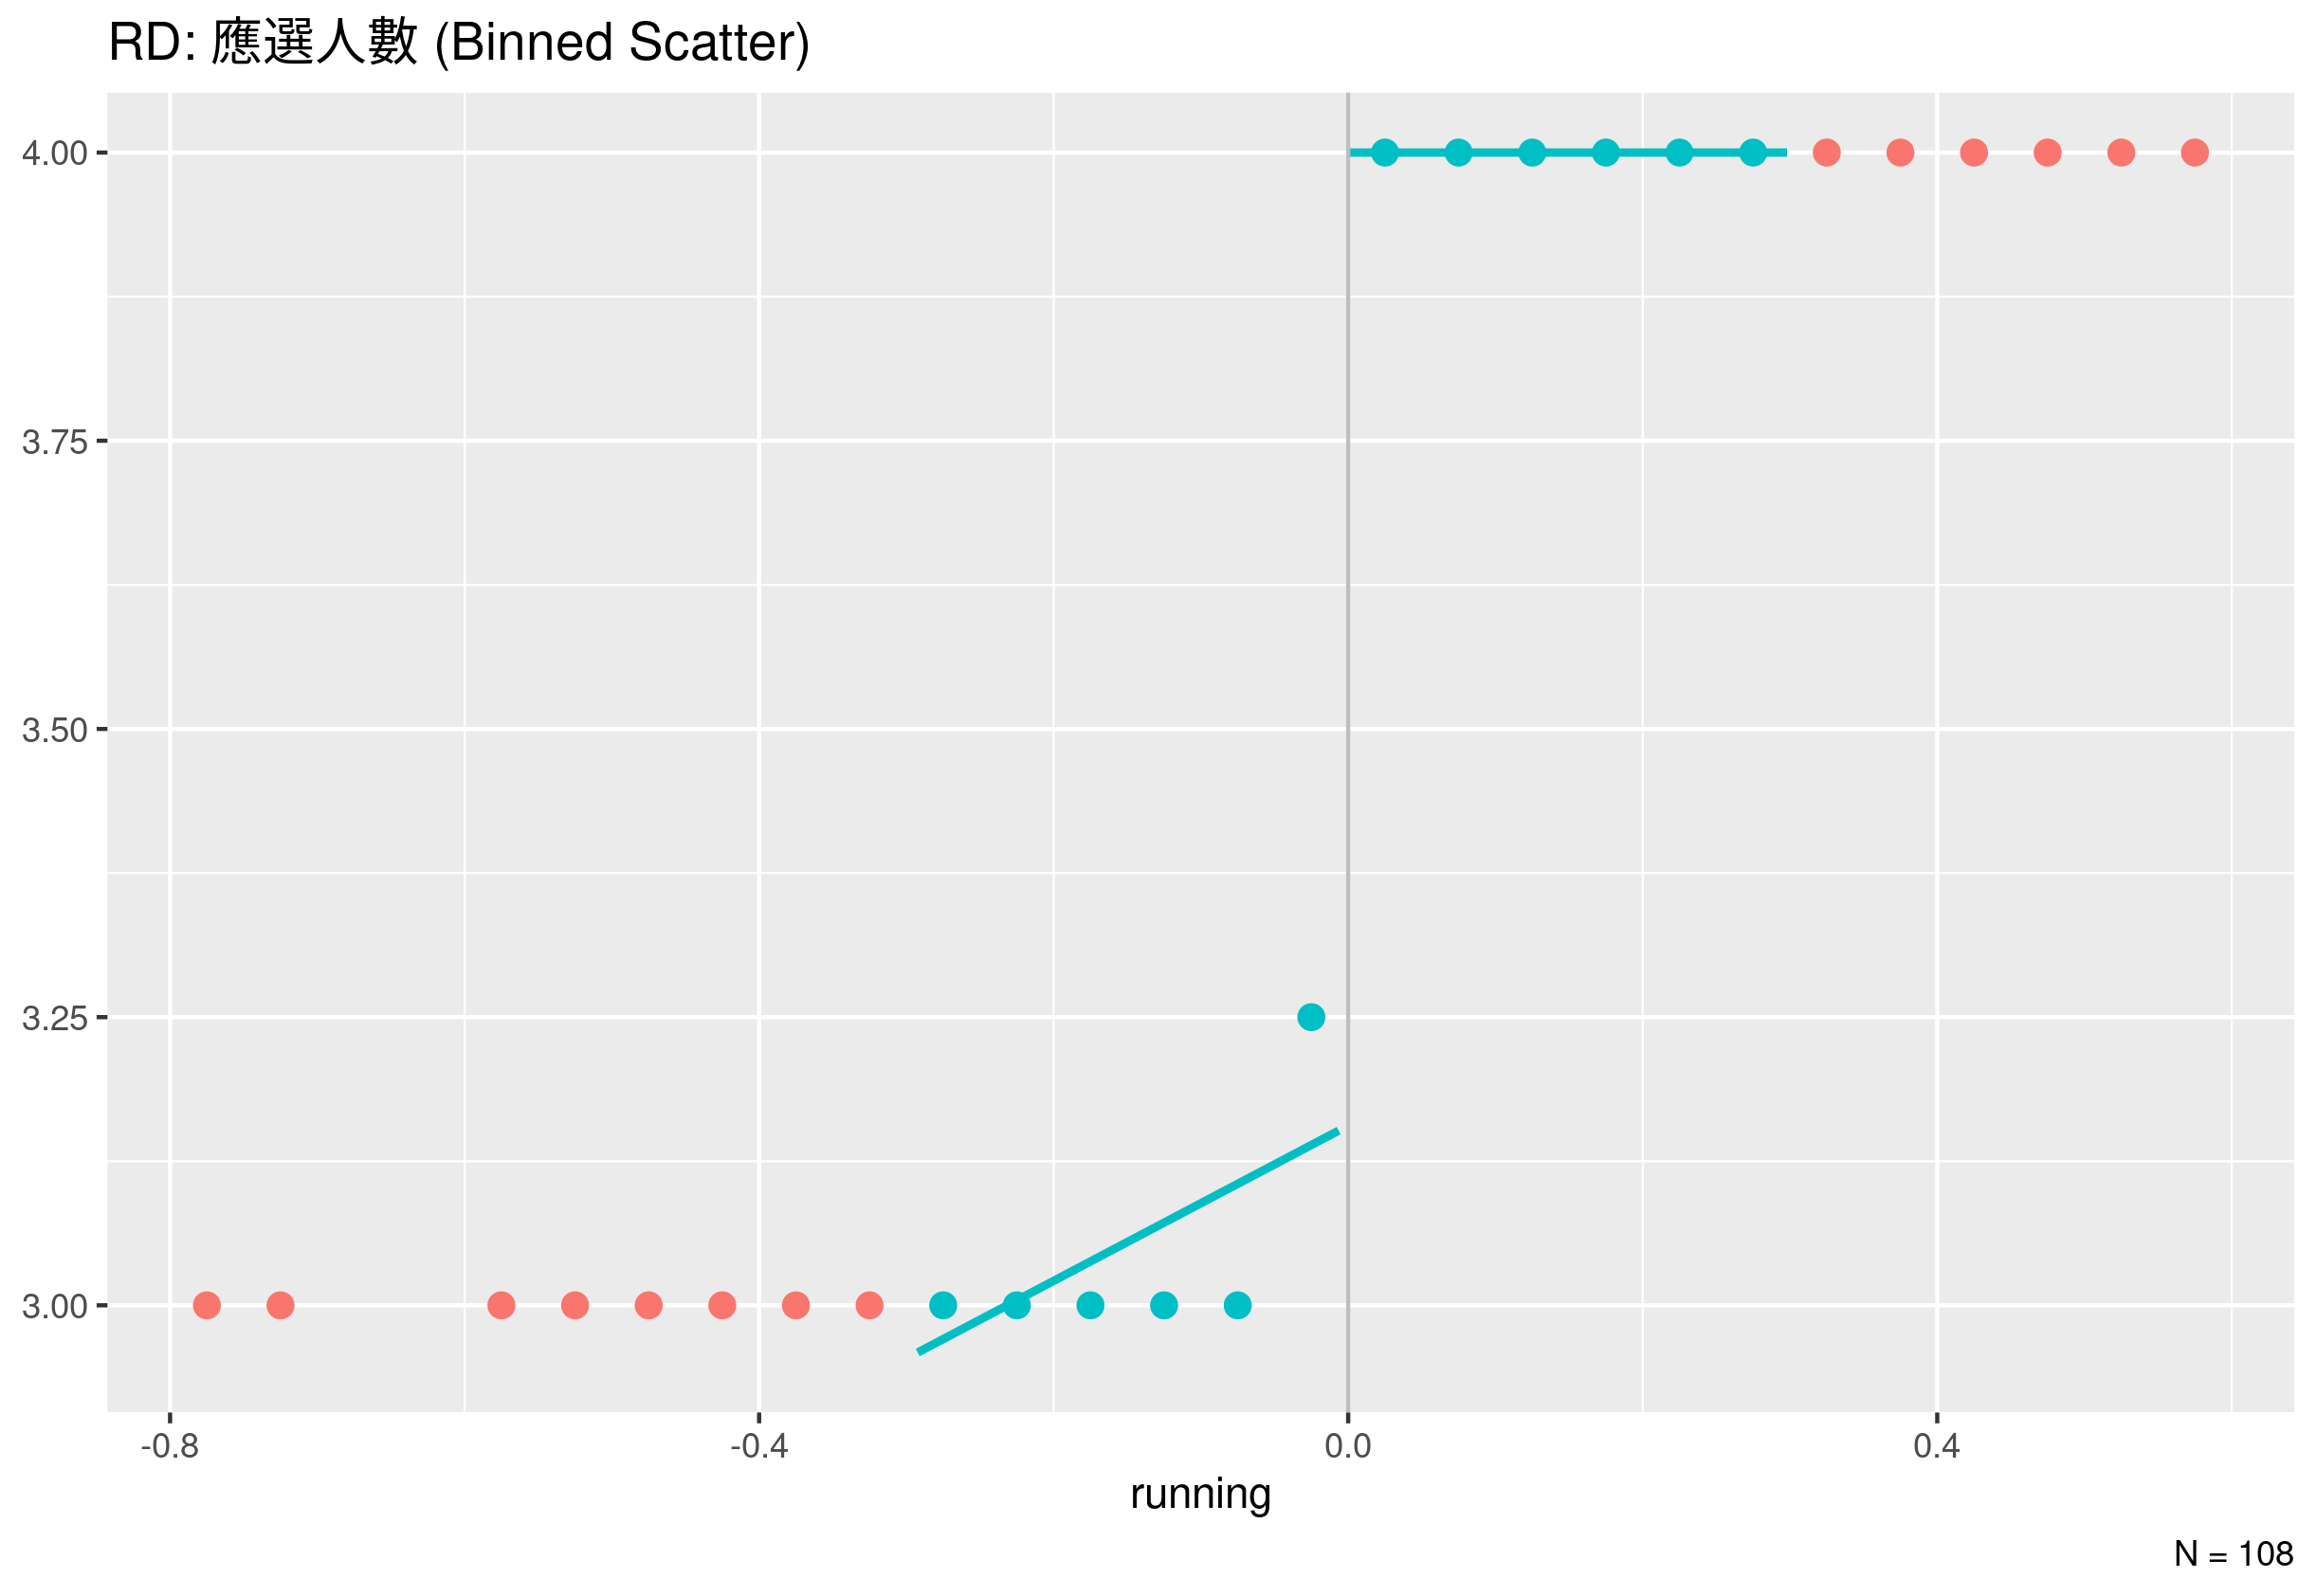
\includegraphics[width=0.9\textwidth,height=\textheight]{assets/3to4.png}
\caption{餘數分配不連續 (3 至 4 席)}
\end{figure}
\end{frame}

\begin{frame}
\begin{block}{1st Stage}
\protect\hypertarget{st-stage}{}
\begin{figure}
\centering
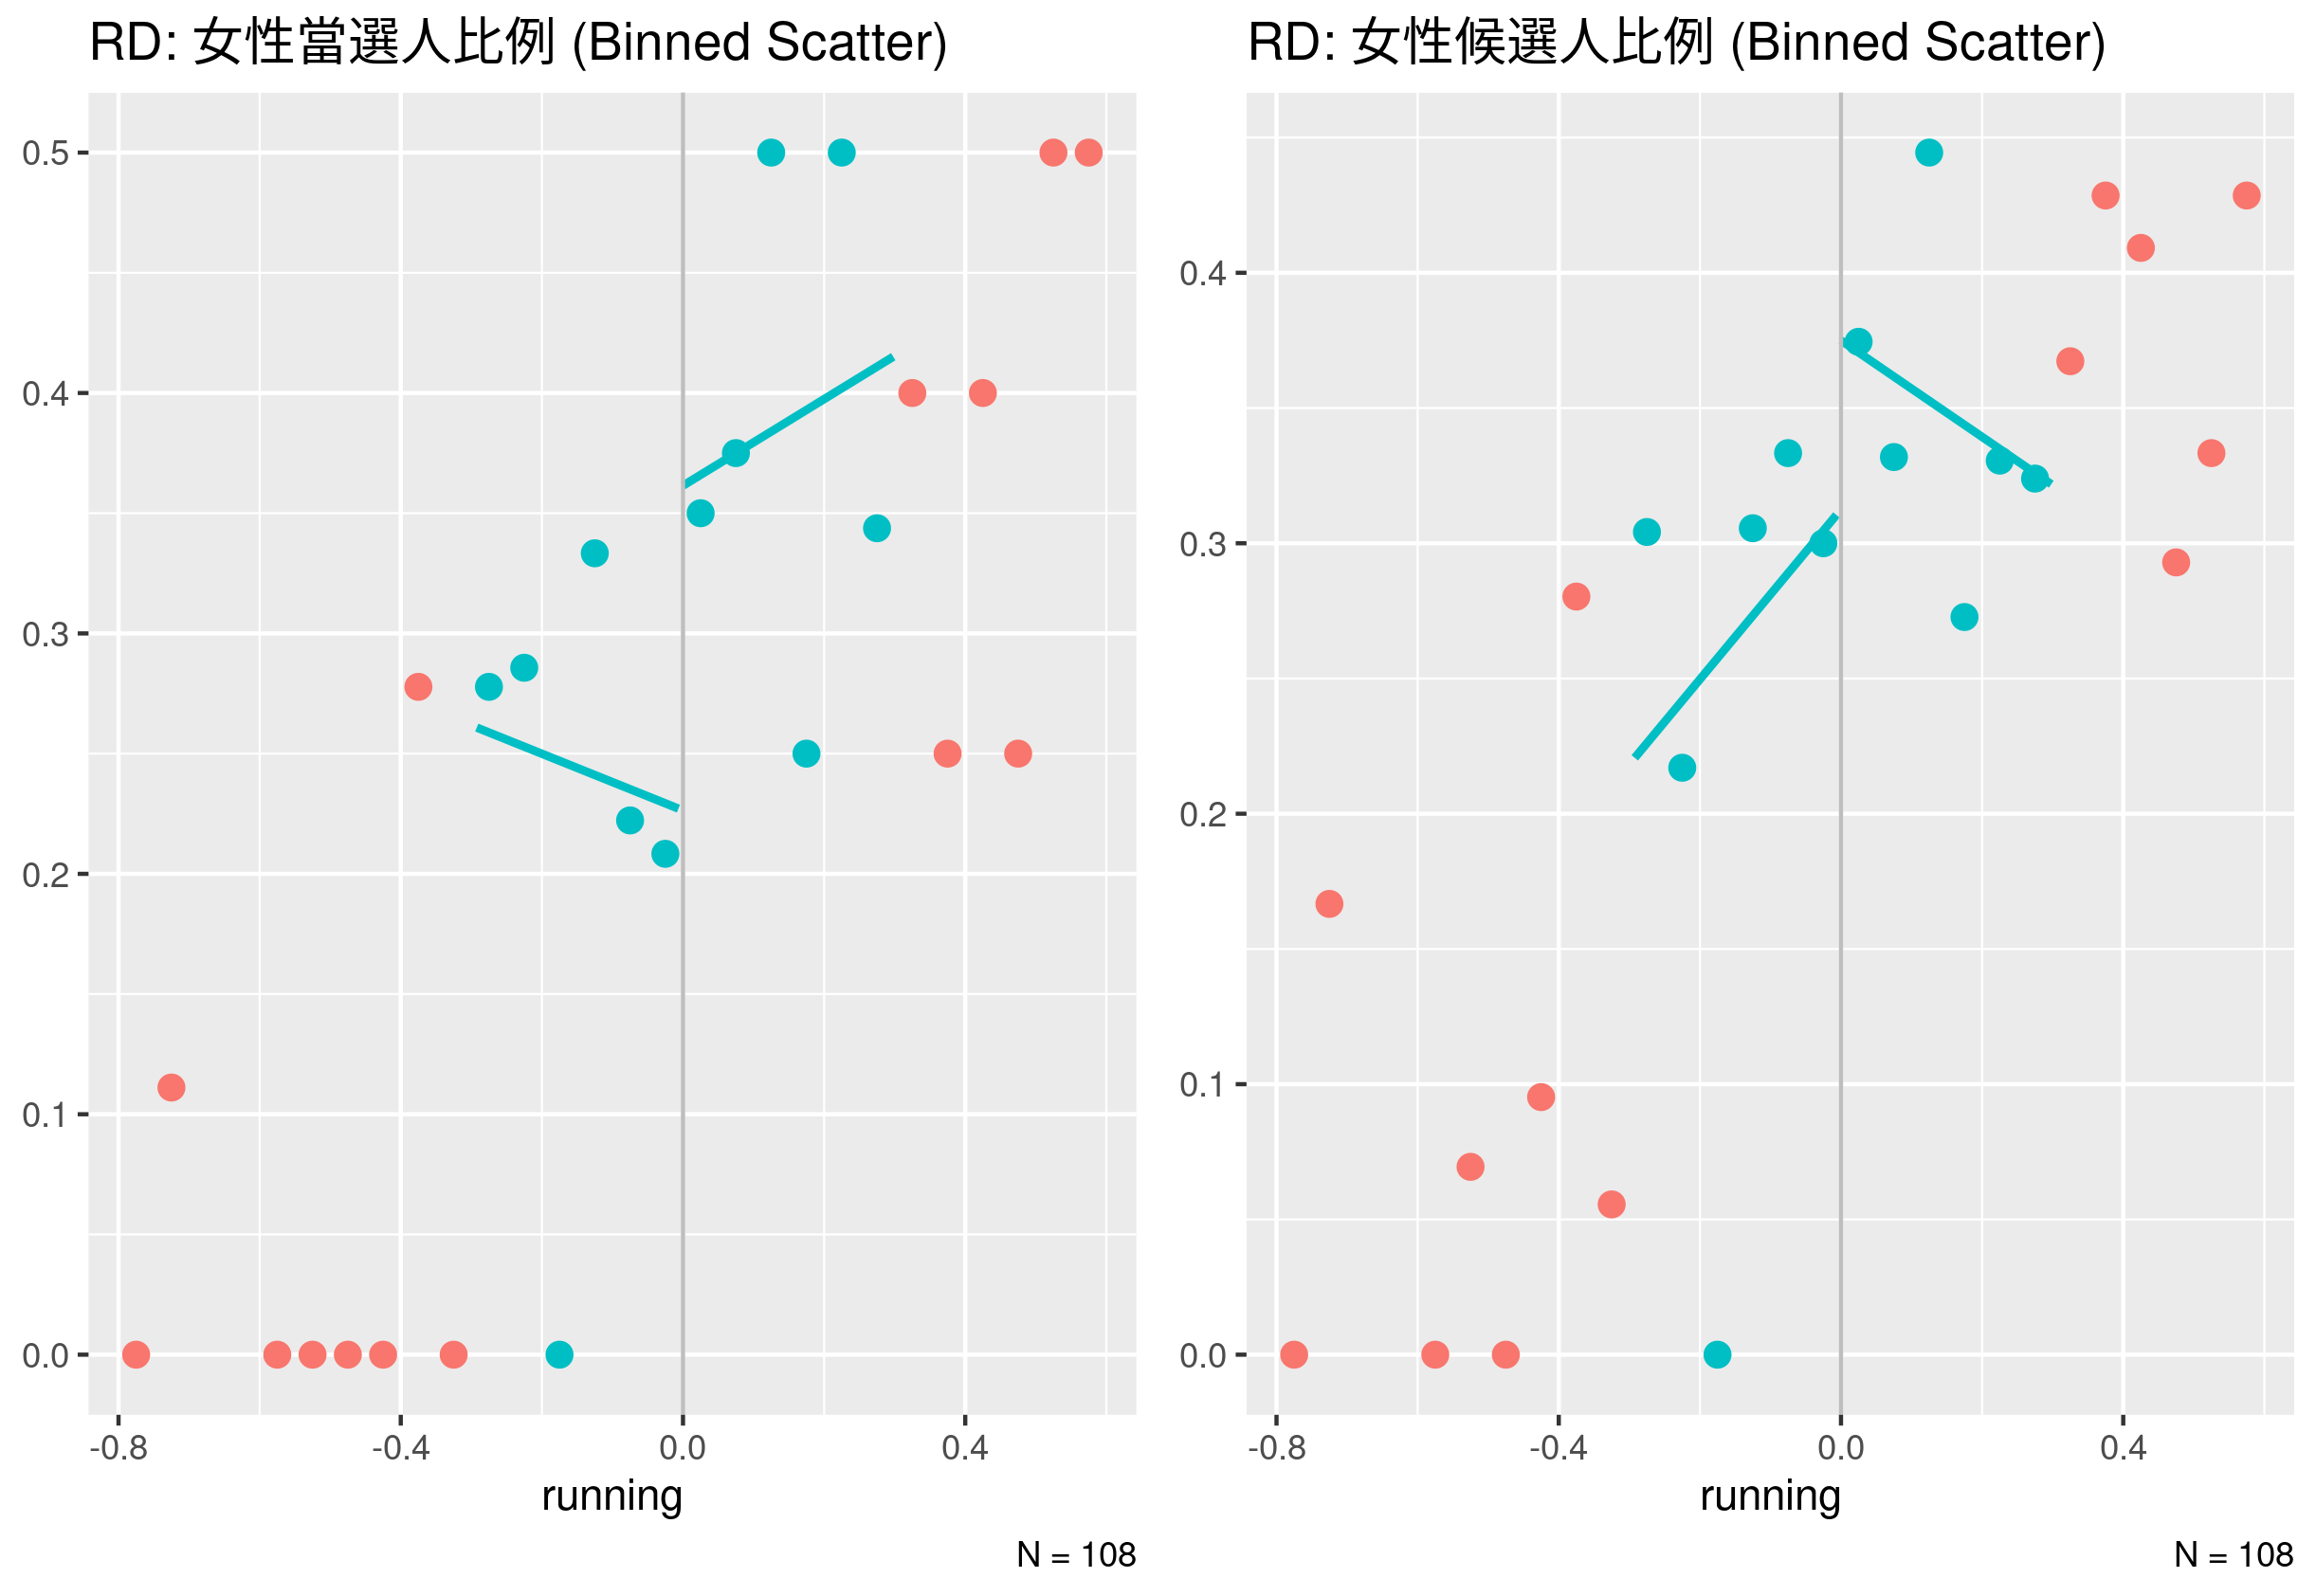
\includegraphics[width=1\textwidth,height=\textheight]{assets/treatments_3to4.png}
\caption{RD 1st Stage (3 至 4 席)}
\end{figure}
\end{block}
\end{frame}

\begin{frame}{應選 \(7 \rightarrow 8\);保障 \(1 \rightarrow 2\)}
\protect\hypertarget{ux61c9ux9078-7-rightarrow-8ux4fddux969c-1-rightarrow-2}{}
\begin{figure}
\centering
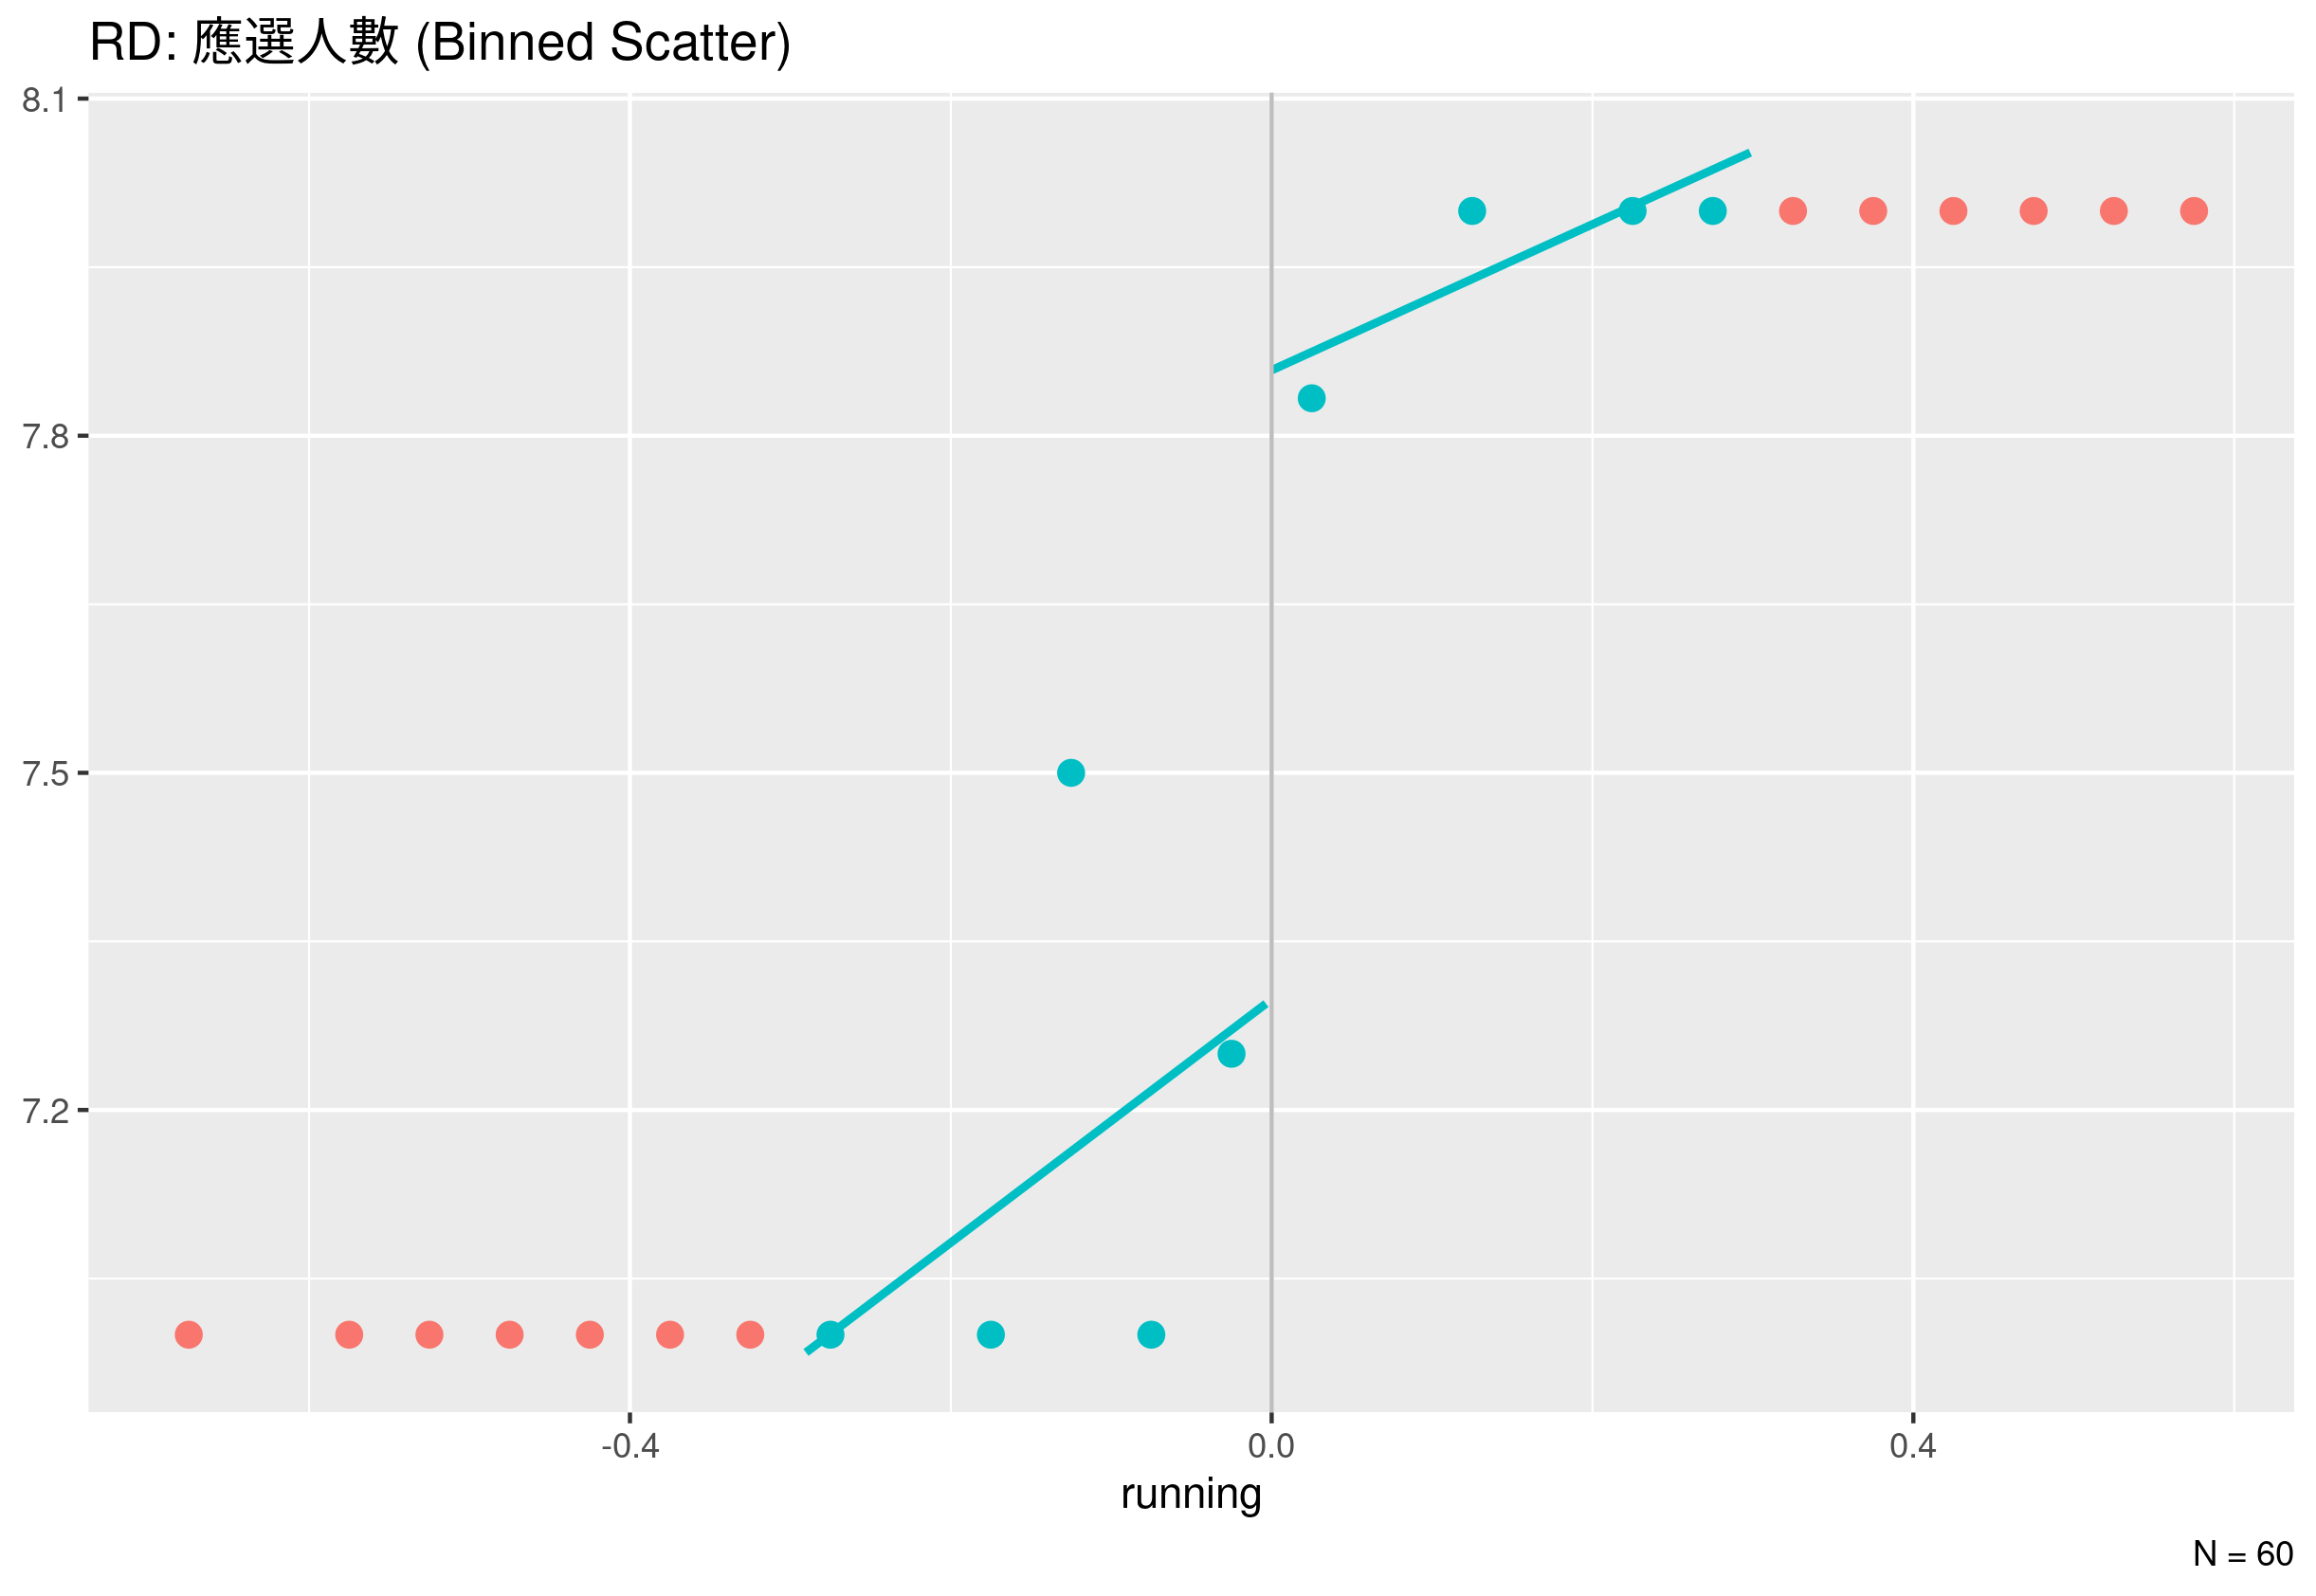
\includegraphics[width=0.9\textwidth,height=\textheight]{assets/7to8.png}
\caption{餘數分配不連續 (7 至 8 席)}
\end{figure}
\end{frame}

\begin{frame}
\begin{block}{1st Stage: 女性當選比例 (Treatment)}
\protect\hypertarget{st-stage-ux5973ux6027ux7576ux9078ux6bd4ux4f8b-treatment}{}
\begin{figure}
\centering
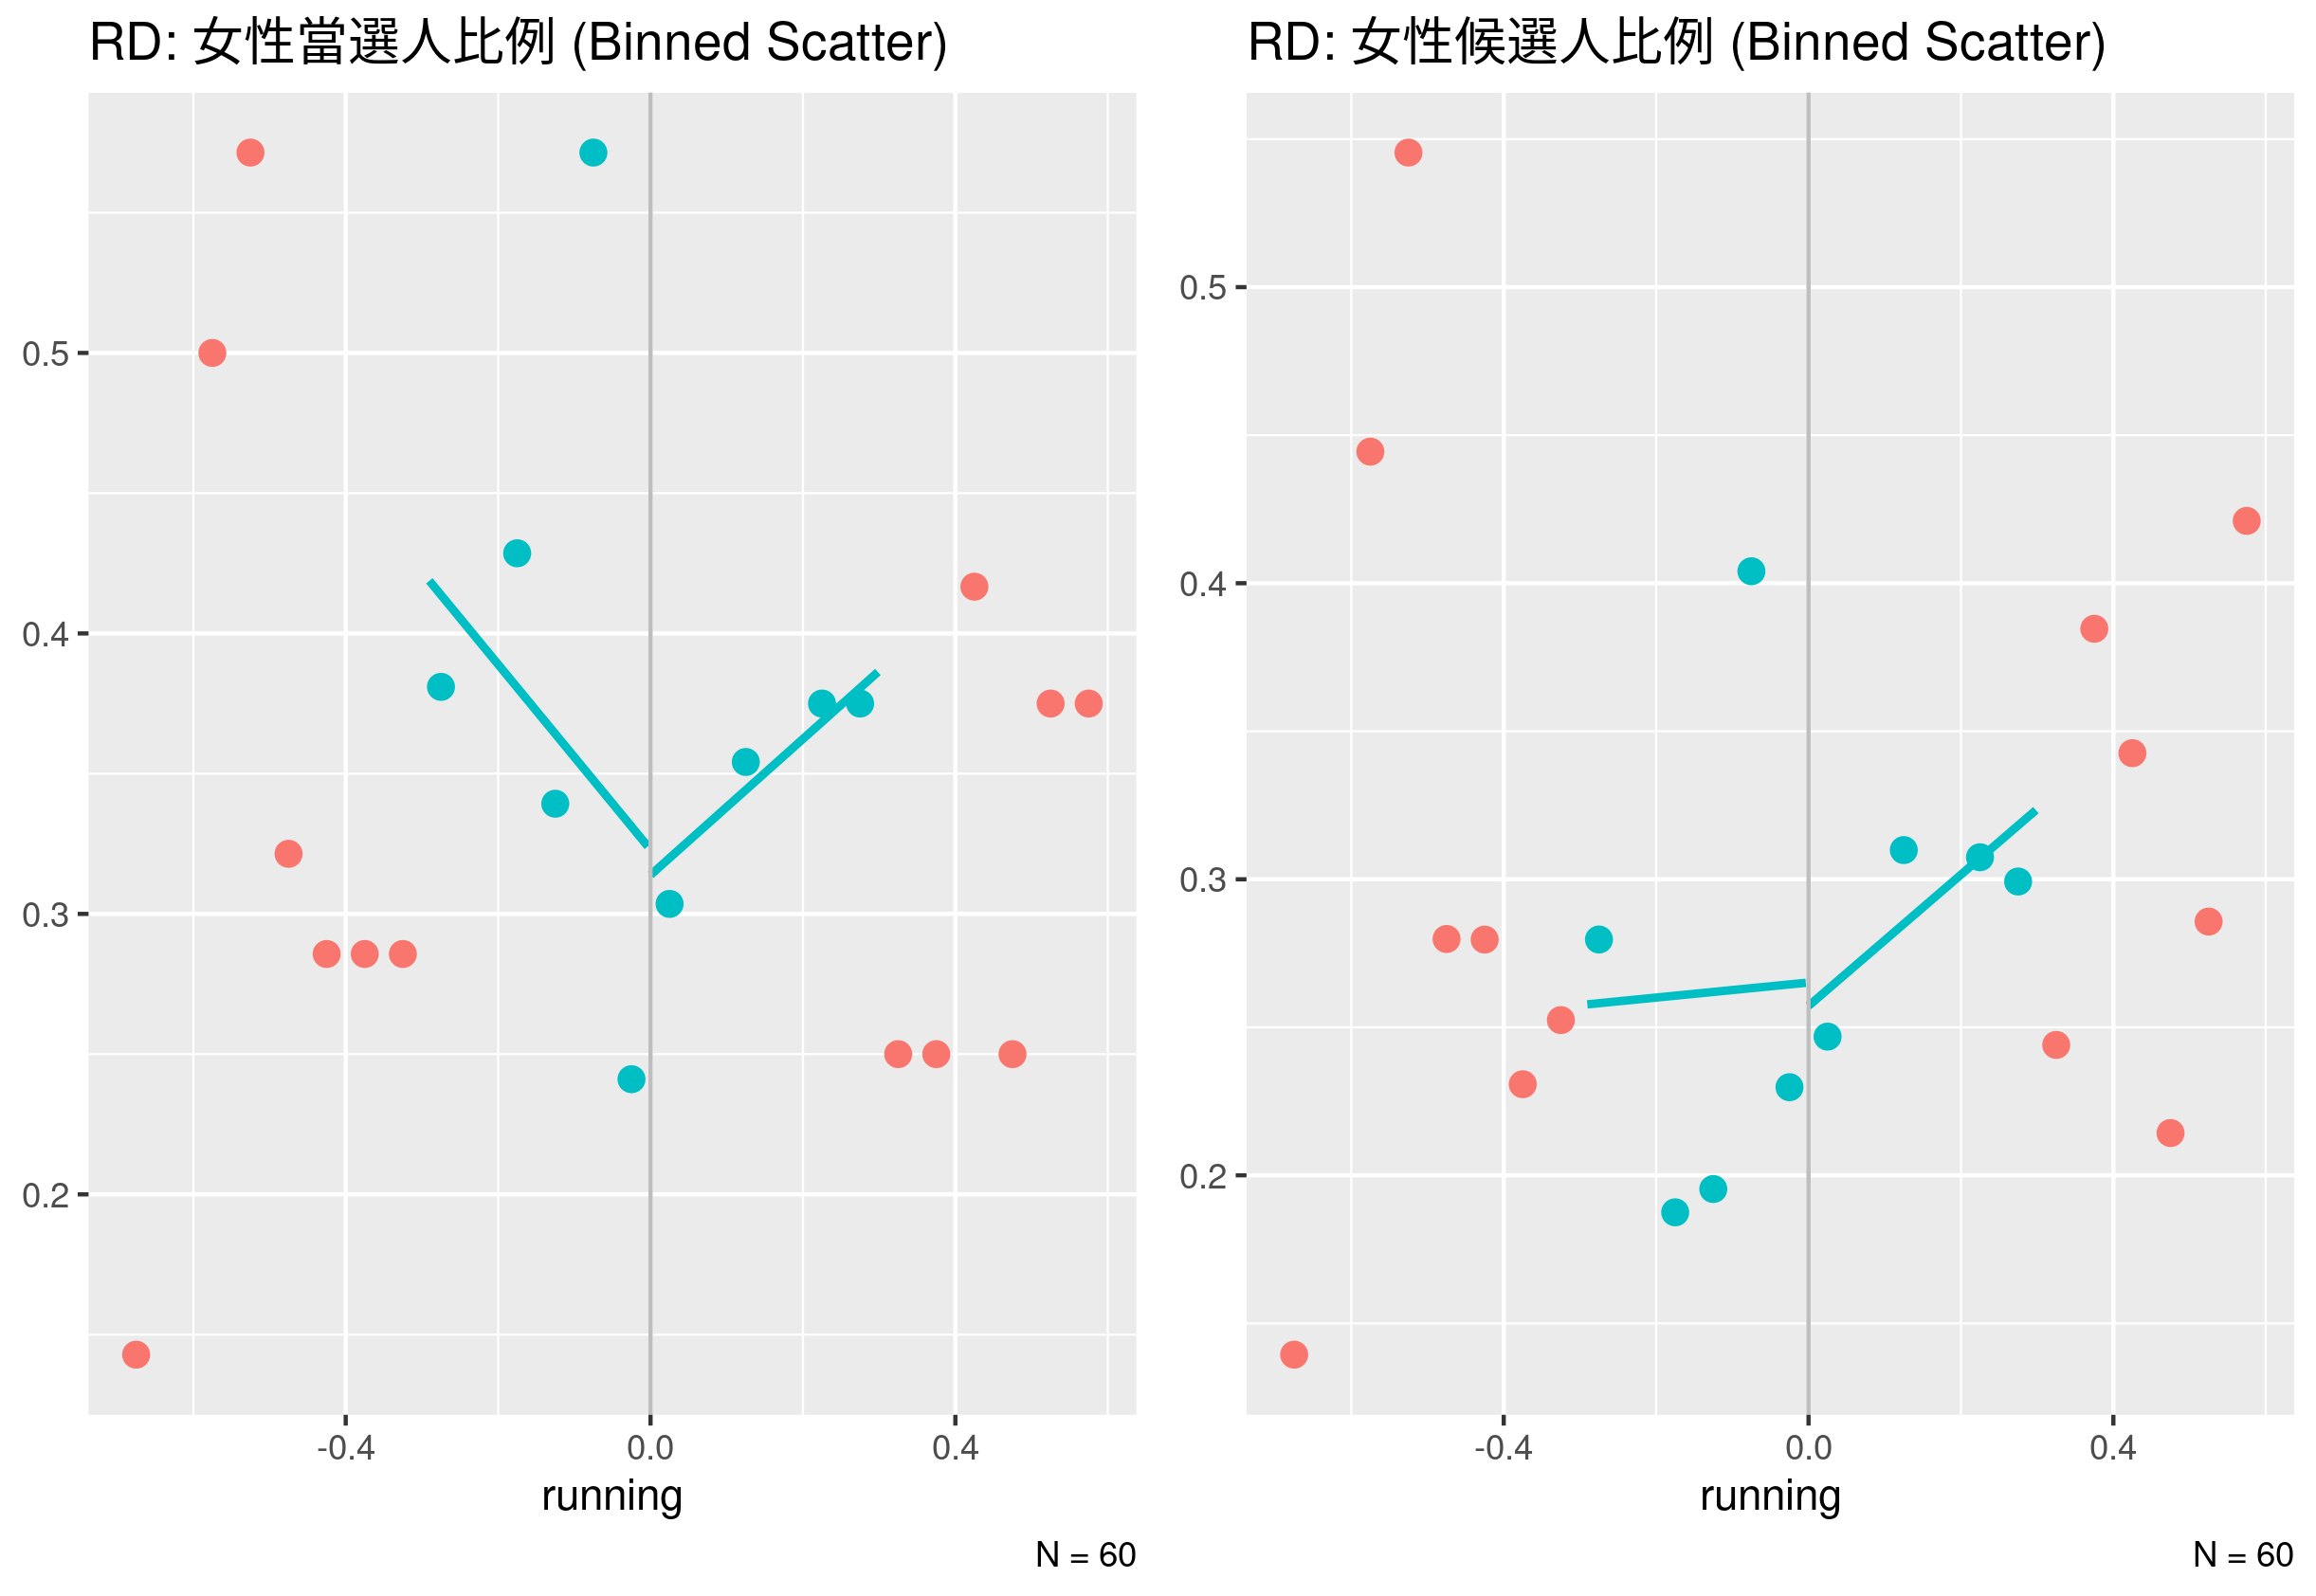
\includegraphics[width=1\textwidth,height=\textheight]{assets/treatments_7to8.png}
\caption{RD 1st Stage (7 至 8 席)}
\end{figure}
\end{block}
\end{frame}

\end{document}
